\chapter{Results and Analysis}
\label{chap5}

In this chapter we perform synthesis of both cores and run the tests described in \autoref{tab:instr_skip_test} and \autoref{tab:coverage_test} using the steps described in \autoref{subsec:sim_glitch}. The waveforms from simulation of the core are shown for all the tests. In every waveform figure the clock signal is on top, the glitched signal is shown in blue and the alert signals are shown in red on the bottom. Results from the synthesis and tests are discussed in \autoref{sec:discussion}.

\section{PPA comparison}
\label{sec:synth_comparison}

Results from synthesis of both cores as well as the number of cycles needed to complete the test program in \autoref{lst:sample_code} are shown in \autoref{tab:ppa_results}. The relative difference from the single core to dual-cores is shown in the table.

\begin{table}[h]
\centering
\caption{PPA results from simulation and synthesis of both setups.}
\label{tab:ppa_results}
\begin{tabular}{c|ccc}
\toprule 
Setup & Area[$pm^2$] & Power[$\mu W$] & Clock Cycles\\
\midrule
\rowcolor{black!20} CV32E40S & 63121.093 & 113.007 & 18424\\
CV32E40DC & 65214.732[$+3.3\%$] & 144.482[$+27.9\%$] & 18415[$-0.05\%$] \\
\bottomrule
\end{tabular}
\end{table}

From the table we see that the area and power consumption are increased by $3.3\%$ and $27.9\%$ respectively. The amount of clock cycles needed to run the test program decreases by $0.05\%$. This is the same decrease achieved from only removing PCH as shown in \autoref{sec:xsecure}.

The amount of clock cycles each core uses to execute the code from \autoref{lst:test_code} and \autoref{lst:coverage_test} is shown in \autoref{tab:test_ccs}. From the table we see that the CV32E40DC uses 9 fewer clock cycles for each of the tests. This amounts to a decrease of $0.32\%$ and $-0.28\%$ for the instruction skipping test and the fault coverage test repspecively. 

\begin{table}[h]
\centering
\caption{Clock cycle used to execute the code in \autoref{lst:test_code} and \autoref{lst:coverage_test} on both cores.}
\label{tab:test_ccs}
\begin{tabular}{c|cc}
\toprule 
Setup & Instruction skipping & Fault coverage \\
\midrule
\rowcolor{black!20} CV32E40S & 2799 & 3132\\
CV32E40DC & 2790[$-0.32\%$] & 3123[$-0.28\%$]\\
\bottomrule
\end{tabular}
\end{table}

\section{Instruction Skipping}
\label{sec:instr_skip_result}

\subsection{CV32E40S}
\label{subsec:single_instr_skip}

\subsubsection{Skipping function call}

The \textit{c.jal} instruction is logged in the \textit{WB} stage at 1752ns. The fault is injected in the \textit{EX} stage at 1743ns. The program counter is glitched to be \textit{0x0000044e}, thus skipping one instruction. 

Glitching of the core was done successfully, and line \textbf{21} in \autoref{lst:test_code} was executed. The waveforms from simulation are shown in \autoref{fig:instr_skip_single_wave}. From the figure one can see that the glitch is detected immediately and a major alert is raised. 

\begin{figure}[h!]
    \centering
    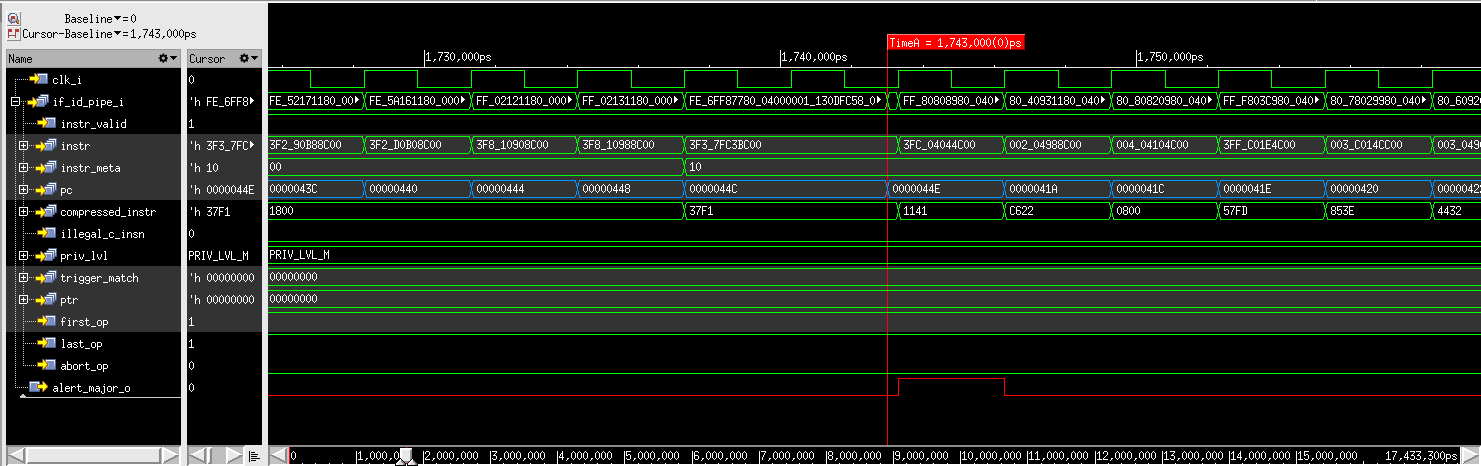
\includegraphics[width=\textwidth]{docs/images/instr_skip_glitch_injection_single_core.png}
    \caption{Waveforms from simulated skip of \textit{c.jal} instruction on CV32E40S.}
    \label{fig:instr_skip_single_wave}
\end{figure}

\subsubsection{Skipping out of while loop}

The \textit{c.j} instruction is logged in the \textit{WB} stage at 1833ns. The fault is injected in the \textit{EX} stage at 1824ns. The program counter is glitched to be \textit{0x0000047c}, thus skipping one instruction.

Glitching out of the while loop was not successful. The attempted instruction skip is detected and a major alert is raised. This can be seen in the simulation waveforms in \autoref{fig:instr_skip_loop_single_wave}. 

\begin{figure}[h!]
    \centering
    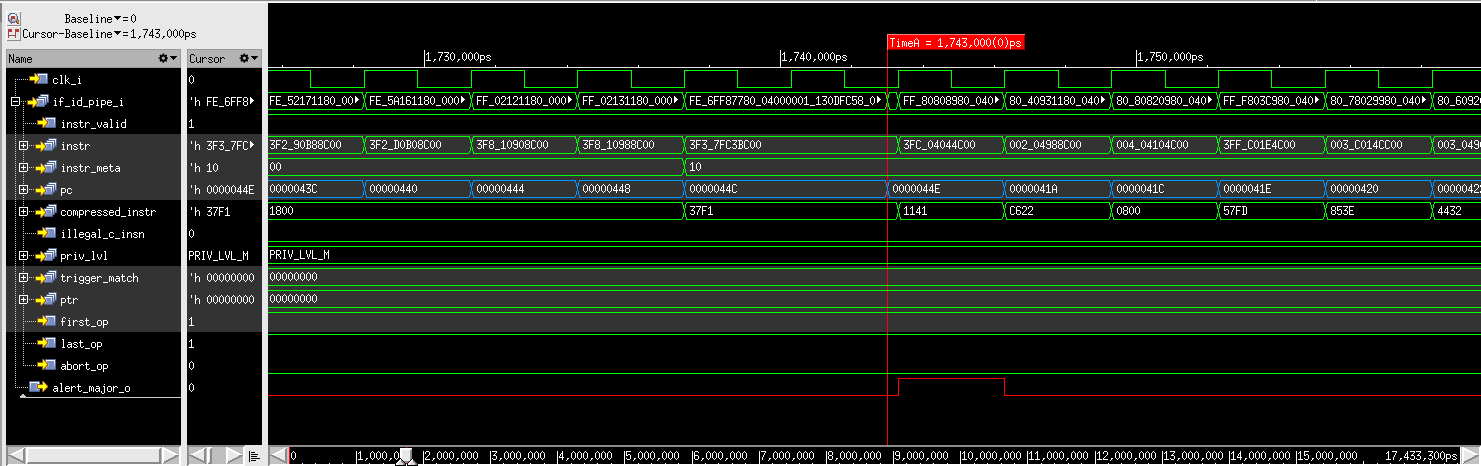
\includegraphics[width=\textwidth]{docs/images/instr_skip_glitch_injection_single_core.png}
    \caption{Waveforms from simulated skip of \textit{c.j} instruction to out of loop on CV32E40S.}
    \label{fig:instr_skip_loop_single_wave}
\end{figure}

\subsubsection{Skipping directly to end}

The call to the \textit{main} function is logged in the \textit{WB} stage at 1737ns. The fault is injected in the \textit{EX} stage at 1728ns. The program counter is glitched to the address \textit{0x00000482}, thus skipping 24 instructions.

This glitch attack was not successful. However, no major alert was raised by the core as can be seen in \autoref{fig:direct_skip_single_wave}. This glitch therefore bypassed the PCH feature. 

\begin{figure}[h!]
    \centering
    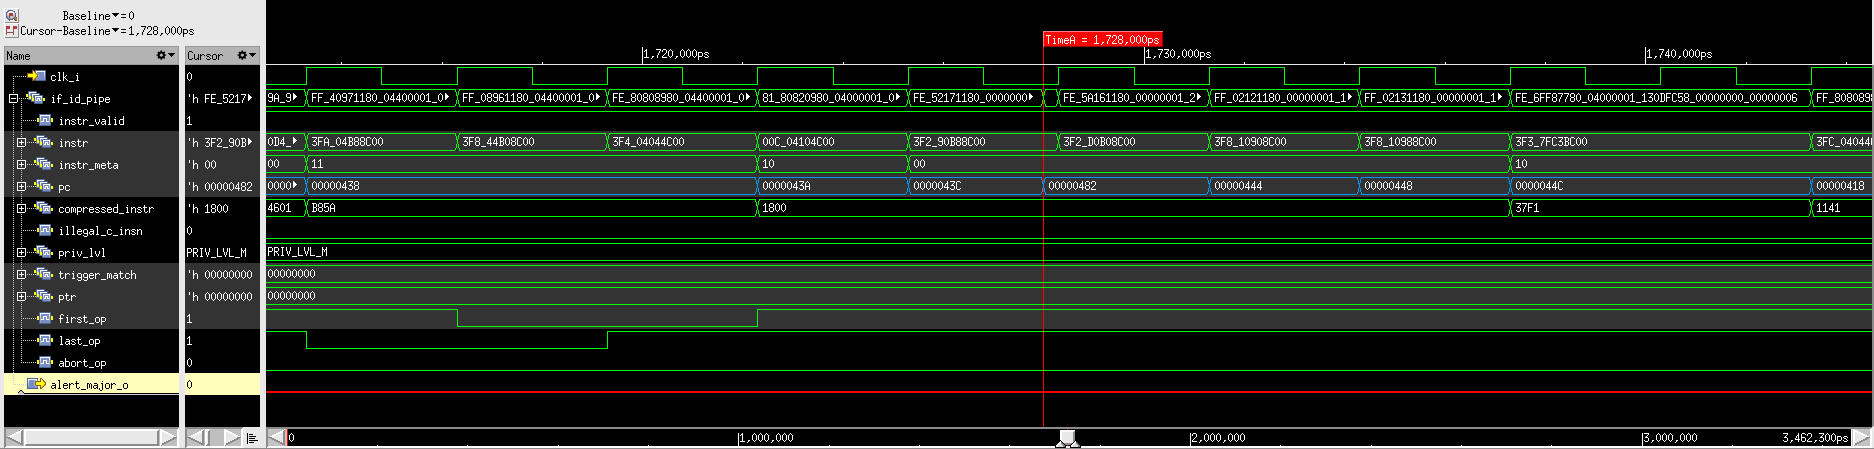
\includegraphics[width=\textwidth]{docs/images/direct_skip_single_core.png}
    \caption{Waveforms from simulated direct instruction skip on CV32E40S.}
    \label{fig:direct_skip_single_wave}
\end{figure}

\subsection{CV32E40DC}
\label{subsec:dual_instr_skip}

\subsubsection{Skipping function call}

The \textit{c.jal} instruction is logged in the \textit{WB} stage at 1707ns. The fault is injected in the \textit{EX} stage at 1698ns. The program counter is glitched to the address \textit{0x0000044e}, thus skipping one instruction. 

The glitch attack was not successful. From \autoref{fig:instr_skip_loop_dual_wave} we observe that the fault is detected immediately and the error propagates through each stage of the pipeline. 

\begin{figure}[h!]
    \centering
    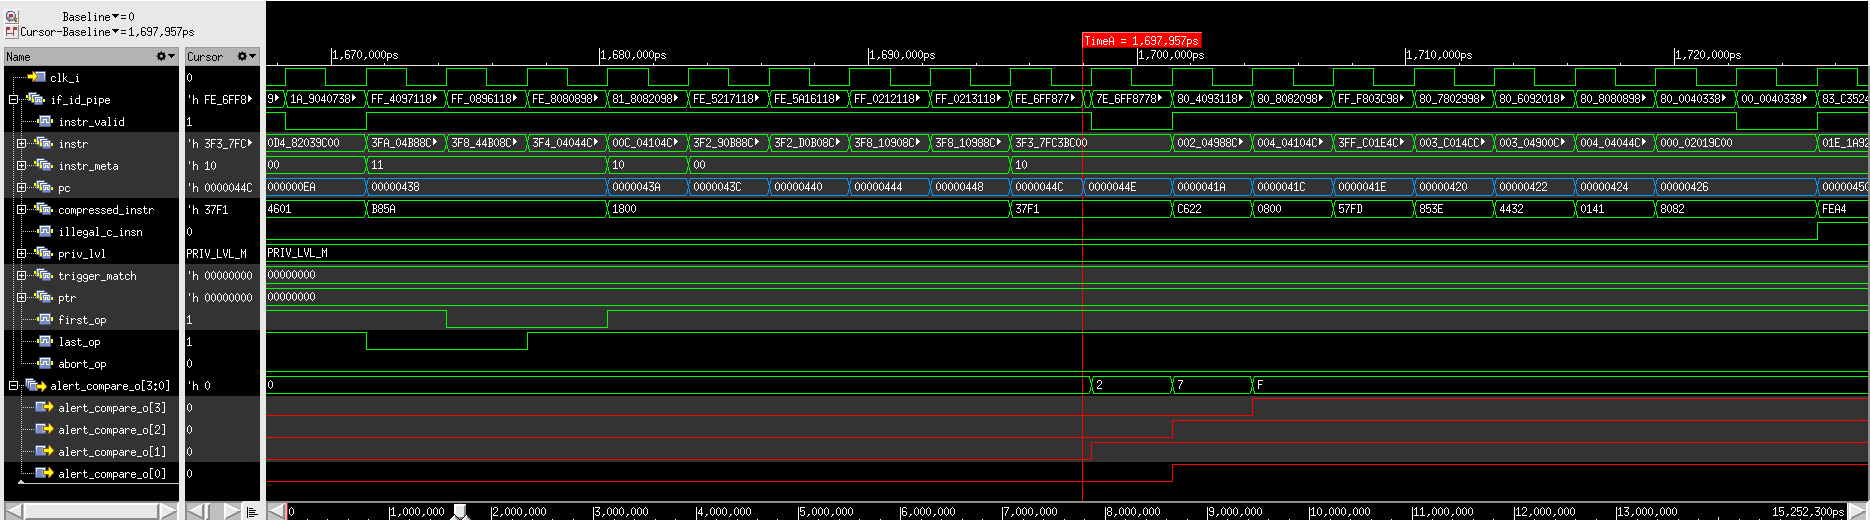
\includegraphics[width=\textwidth]{docs/images/instr_skip_dual_core.png}
    \caption{Waveforms from simulated skip of \textit{c.jal} instruction on CV32E40DC.}
    \label{fig:instr_skip_dual_wave}
\end{figure}


\subsubsection{Skipping out of while loop}

The \textit{c.j} instruction is logged in the \textit{WB} stage at 1782ns. The fault is injected in the \textit{EX} stage at 1773ns. The program counter is glitched to the address \textit{0x0000047c}, skipping one instruction.

The glitch attack was not successful. From \autoref{fig:instr_skip_loop_dual_wave} we observe that the fault is detected immediately and the error propagates though each stage of the pipeline. 

\begin{figure}[h!]
    \centering
    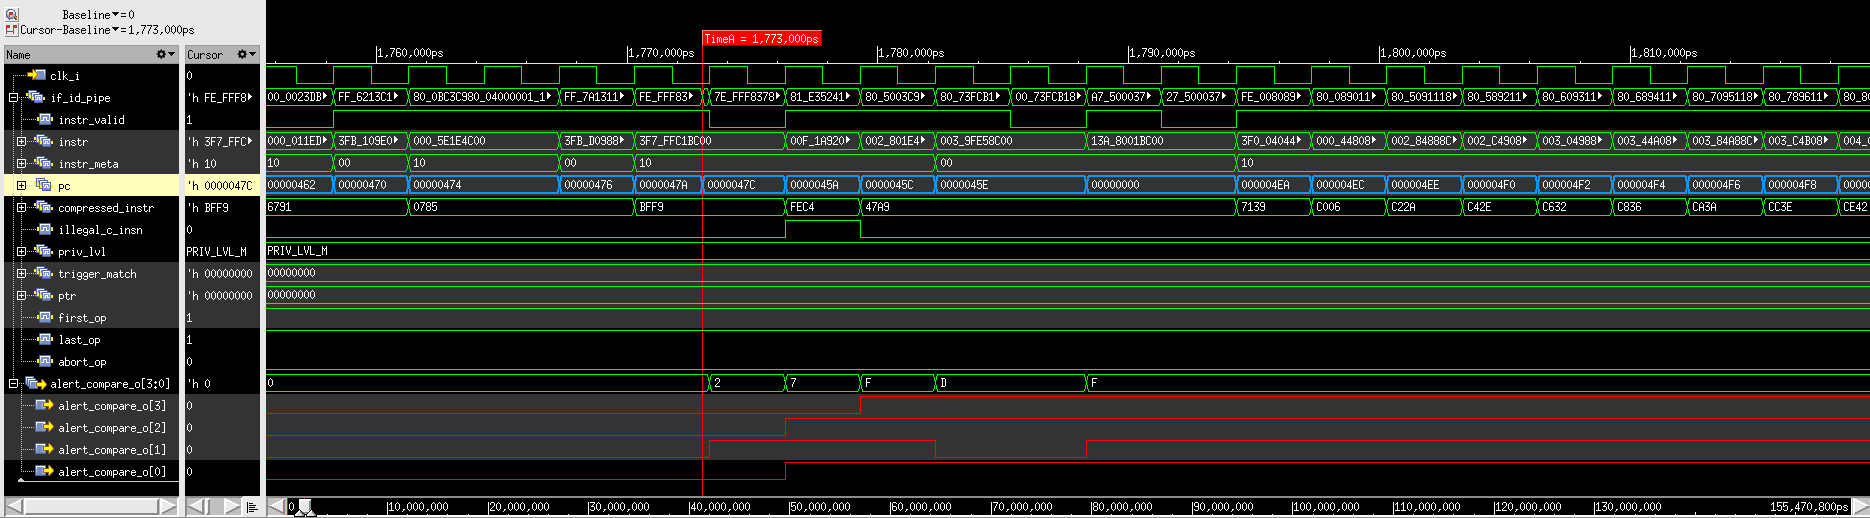
\includegraphics[width=\textwidth]{docs/images/instr_skip_loop_dual_core.png}
    \caption{Waveforms from simulated skip of \textit{c.j} instruction to jump out of loop on CV32E40DC.}
    \label{fig:instr_skip_loop_dual_wave}
\end{figure}

\subsubsection{Skipping directly to end}

The call to the \textit{main} function is logged in the \textit{WB} stage at 1689ns. The fault is injected in the \textit{EX} stage at 1680ns. The program counter is glitched to the address \textit{0x00000482}, thus skipping 24 instructions.

The glitch attack was not successful. From \autoref{fig:direct_skip_dual_wave} we observe that the fault is detected immediately and the error propagates through each stage of the pipeline. 

\begin{figure}[h!]
    \centering
    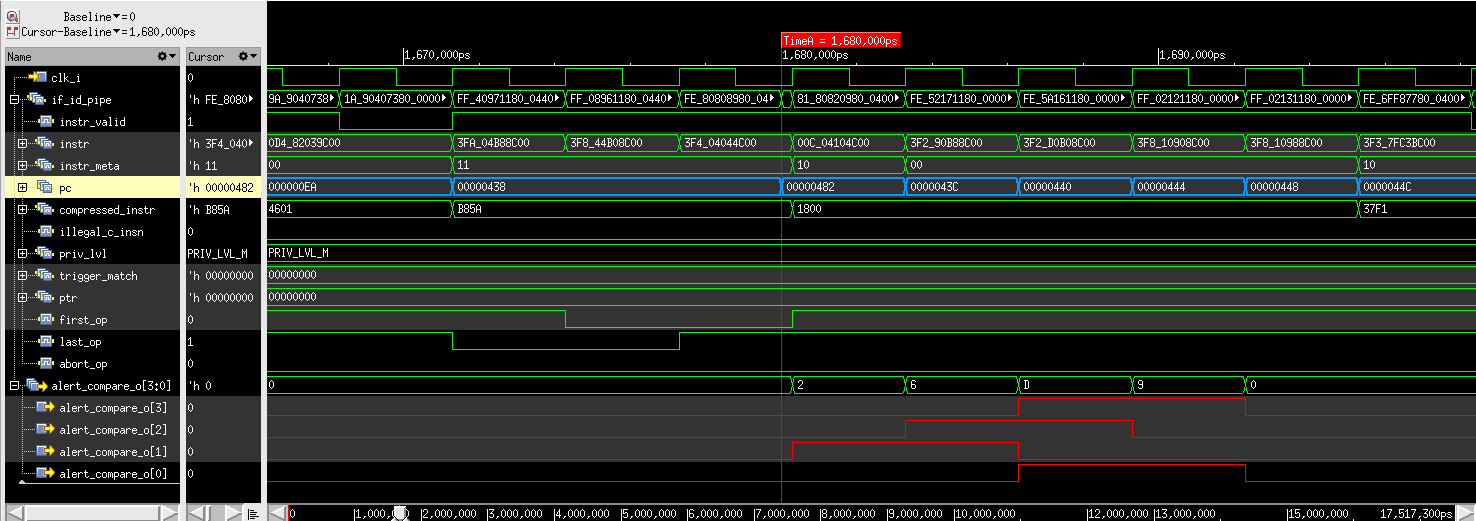
\includegraphics[width=\textwidth]{docs/images/direct_skip_dual_core.png}
    \caption{Waveforms from simulated direct instruction skip on CV32E40DC.}
    \label{fig:direct_skip_dual_wave}
\end{figure}


\section{Coverage Test}
\label{sec:cov_test_result}

\subsection{CV32E40S}

\subsubsection{Glitching load instruction}

The \textit{lw} instruction is logged in the \textit{WB} stage at 1827ns. The fault is also injected at 1827ns. The glitch attack was successful and the wrong value for the Fibonacci number was calculated. From \autoref{fig:lw_glitch_single_wave} we see that no major alert was raised by the single core, and the glitch goes undetected. 

\begin{figure}[h!]
    \centering
    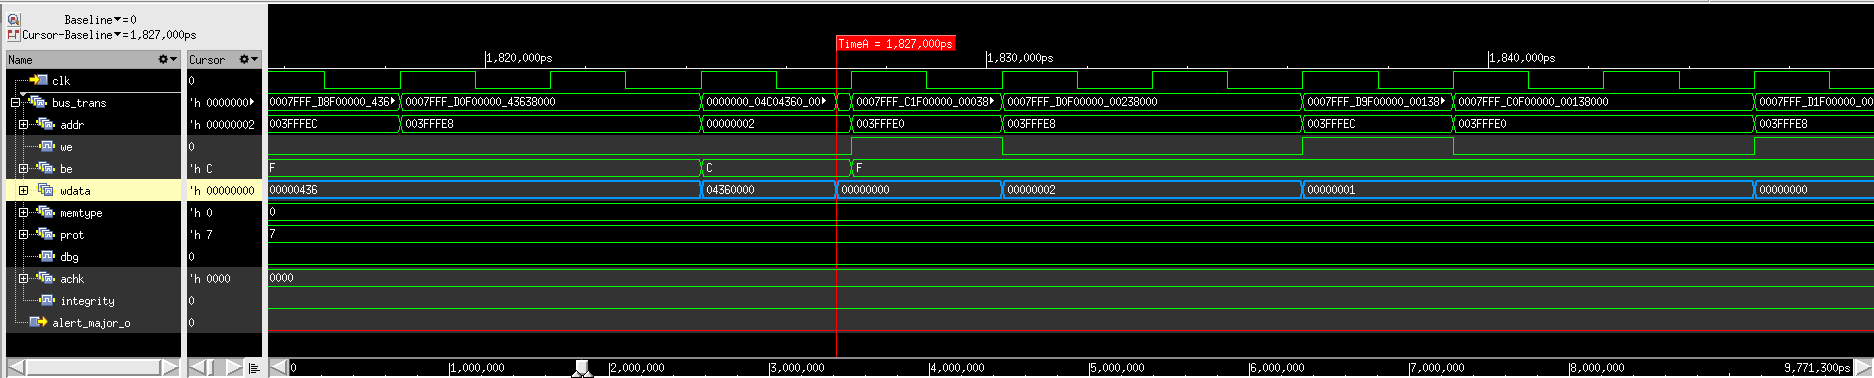
\includegraphics[width=\textwidth]{docs/images/lw_glitch_single_core.png}
    \caption{Waveforms from simulated glitched LW instruction skip on CV32E40S.}
    \label{fig:lw_glitch_single_wave}
\end{figure}

\subsubsection{Glitching store instruction}

The \textit{sw} instruction is logged in the \textit{WB} stage at 1836ns. The fault is also injected at 1836ns. The glitch attack was successful and the wrong value for the Fibonacci number was calculated. From \autoref{fig:sw_glitch_single_wave} we see that no major alert was raised by the single core, and the glitch goes undetected. 

\begin{figure}[h!]
    \centering
    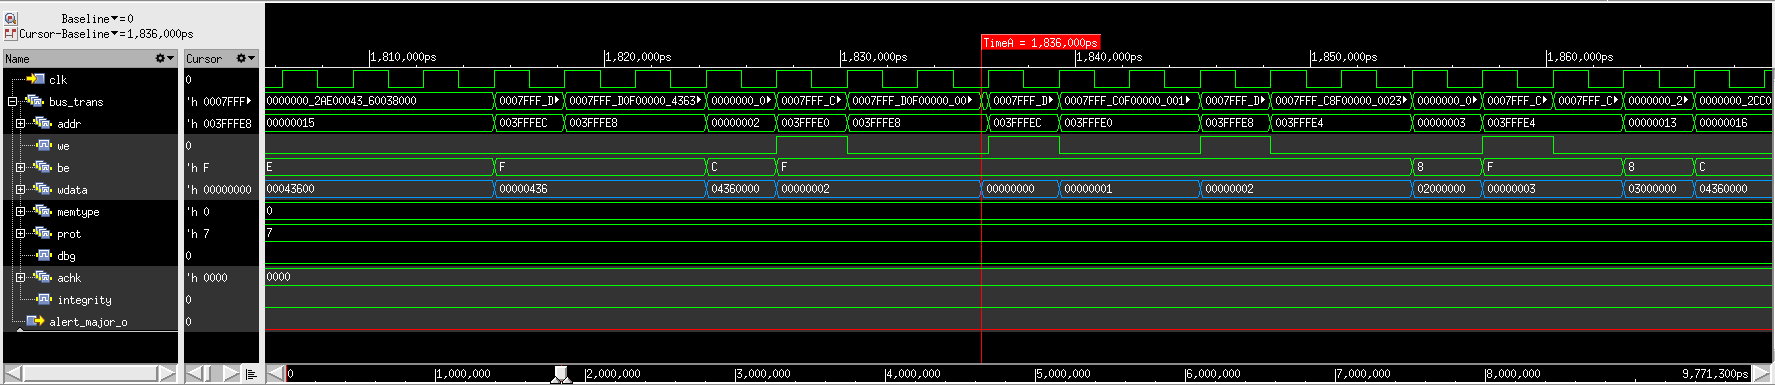
\includegraphics[width=\textwidth]{docs/images/sw_glitch_single_core.png}
    \caption{Waveforms from simulated glitched SW instruction skip on CV32E40S.}
    \label{fig:sw_glitch_single_wave}
\end{figure}


\subsection{Dual-Core Lockstep}

\subsubsection{Glitching load instruction}

The \textit{lw} instruction is logged in the \textit{WB} stage at 1722ns. The fault is also injected at 1722ns. The glitch attack was successful and the wrong value for the Fibonacci number was calculated. From \autoref{fig:lw_glitch_dual_wave} we see that bit \textit{0} on the \textit{alert\_compare\_o} bus is raised, meaning the system has detected a glitch in an OBI interface. 

\begin{figure}[h!]
    \centering
    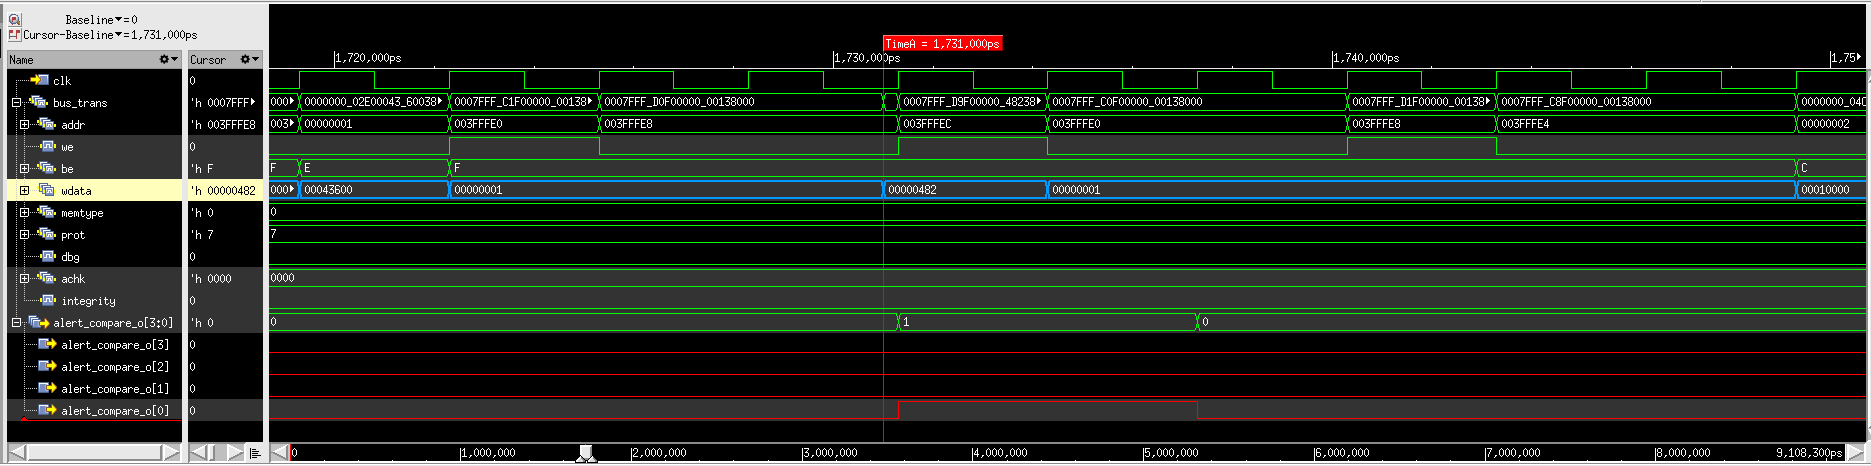
\includegraphics[width=\textwidth]{docs/images/lw_glitch_dual_core.png}
    \caption{Waveforms from simulated glitched LW instruction skip on Dual-Core Lockstep setup.}
    \label{fig:lw_glitch_dual_wave}
\end{figure}

\subsubsection{Glitching store instruction}

The \textit{sw} instruction is logged in the \textit{WB} stage at 1731ns. The fault is also injected at 1731ns. The glitch attack was successful and the wrong value for the Fibonacci number was calculated. From figure \autoref{fig:sw_glitch_dual_wave} we see that bit \textit{0} on the \textit{alert\_compare\_o} bus is raised, meaning the system has detected a glitch in an OBI interface. 

\begin{figure}[h!]
    \centering
    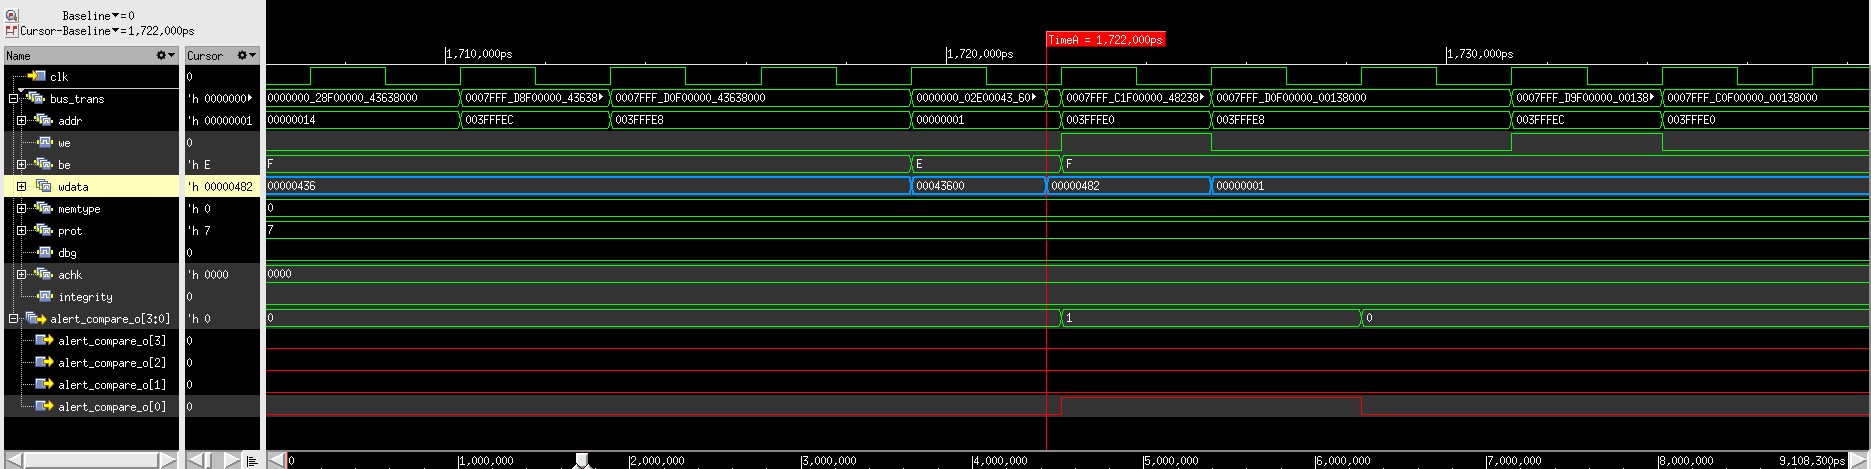
\includegraphics[width=\textwidth]{docs/images/sw_glitch_dual_core.png}
    \caption{Waveforms from simulated glitched SW instruction skip on Dual-Core Lockstep setup.}
    \label{fig:sw_glitch_dual_wave}
\end{figure}

\section{Discussion}
\label{sec:discussion}

As discussed in \autoref{sec:xsecure}, removing the PCH feature from the \textit{Xsecure} extension would lead to an increase in execution speed as shown in \autoref{tab:ppa_results} and \autoref{tab:test_ccs}. However, as mentioned previously this increase is limited by the side-channel attack prevention that also exists within the core. Exactly why the decrease in clock cycles from the CV32E40S to the CV32E40DC is always 9 is yet to be determined. This is not explained in the documentation for the core.  

Adding an extra core is also shown to add area and power usage. The increase in area is however smaller than the increase in power usage relative to the CV3E40S. The reason for this is that the CV32E40DC mainly adds computationally heavy logic circuits. These circuits will not necessarily occupy a lot area, but they do have a non-negligible dynamic power consumption.  

Detecting instruction skips is shown to be more reliable in the Dual-Core Lockstep setup as this was able to detect a glitch in all three test cases. The regular single core was only able to detect a glitch in two of the three tests, and the direct skipping glitch went undetected. For unknown reasons, the function call skipping glitch was only successful in the single core setup. This glitch could be repeated successfully and was therefore not random. The reason for this could be due to some difference in timing between the single and dual-core.

For the coverage test it is clear that the Dual-Core Lockstep setup outperforms the single core as it is able to detect both glitch attacks, where as the single core detects neither of them. 